% Header trang
\noindent
{\small\textbf{184} \quad \textbf{\textsf{CHƯƠNG 3}} \quad \textsf{Các quy tắc tính đạo hàm}}
\vspace{10pt}

% PHẦN BÀI TẬP TRÊN: 2 CỘT
\noindent
\begin{minipage}[t]{0.48\textwidth}
  \noindent\textbf{85.} Cho
  \[
  f(x) = \begin{cases}
    x^2 & \text{nếu } x \le 2 \\
    mx + b & \text{nếu } x > 2
  \end{cases}
  \]
  Tìm các giá trị của $m$ và $b$ để $f$ khả vi tại mọi điểm.

  \vspace{10pt}
  \noindent\textbf{86.} Tìm các số $a$ và $b$ sao cho hàm số đã cho $g$ khả vi tại $1$.
  \[
  g(x) = \begin{cases}
    ax^3 - 3x & \text{nếu } x \le 1 \\
    bx^2 + 2 & \text{nếu } x > 1
  \end{cases}
  \]

  \vspace{8pt}
  \noindent\textbf{87.} Tính $\displaystyle \lim_{x \to 1} \frac{x^{1000} - 1}{x - 1}$.

  \vspace{12pt}
  \noindent\textbf{88.} Một tiếp tuyến được vẽ tới hyperbol $xy = c$ tại một điểm $P$ như minh họa trong hình vẽ.
  \begin{enumerate}[label=(\alph*), leftmargin=*, itemsep=2pt, topsep=3pt]
    \item Chứng minh rằng trung điểm của đoạn thẳng bị chắn trên tiếp tuyến này bởi các trục tọa độ chính là $P$.
  \end{enumerate}
\end{minipage}%
\hfill
\begin{minipage}[t]{0.48\textwidth}
  \begin{enumerate}[label=(\alph*), leftmargin=*, itemsep=2pt, topsep=0pt, start=2]
    \item Chứng minh rằng tam giác tạo bởi tiếp tuyến và các trục tọa độ luôn có cùng một diện tích, bất kể điểm $P$ nằm ở vị trí nào trên hyperbol.
  \end{enumerate}

  \begin{center}
    \vspace{-2pt}
    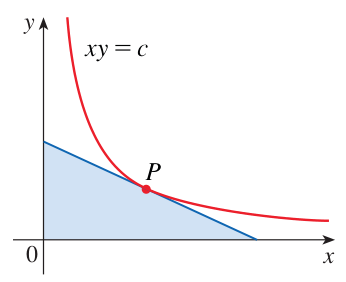
\includegraphics[width=0.54\linewidth]{images/p0219_fig1.png}
    \vspace{-2pt}
  \end{center}

  \noindent\textbf{89.} Vẽ sơ đồ minh họa hai đường thẳng vuông góc cắt nhau trên trục $y$ và đều tiếp xúc với parabol $y = x^2$. Hai đường thẳng này cắt nhau tại điểm nào?

  \vspace{8pt}
  \noindent\textbf{90.} Phác thảo các parabol $y = x^2$ và $y = x^2 - 2x + 2$. Bạn có nghĩ rằng tồn tại một đường thẳng tiếp xúc với cả hai đường cong này không? Nếu có, hãy tìm phương trình của nó. Nếu không, hãy giải thích lý do.

  \vspace{8pt}
  \noindent\textbf{91.} Nếu $c > \frac{1}{2}$, có bao nhiêu đường thẳng đi qua điểm $(0, c)$ là đường pháp tuyến của parabol $y = x^2$? Điều gì xảy ra nếu $c \le \frac{1}{2}$?
\end{minipage}

\vspace{18pt}

% DỰ ÁN ỨNG DỤNG
\begin{tcolorbox}[
  enhanced,
  colback=projectbg,
  colframe=bordergreen,
  boxrule=0.6pt,
  arc=0mm,
  left=8pt, right=8pt, top=6pt, bottom=8pt
]
  % Tiêu đề Dự án
  \noindent
  \begin{minipage}{\linewidth}
    \centering
    \decorativelines{0.07\linewidth}
    \hspace{5pt}
    {\bfseries\sffamily\color{bannergreen} DỰ ÁN ỨNG DỤNG}
    \hspace{5pt}\vline width 0.8pt height 10pt depth 2pt\hspace{7pt}
    {\bfseries\sffamily\color{darkslate} XÂY DỰNG TÀU LƯỢN SIÊU TỐC TỐT HƠN}
    \hspace{5pt}
    \decorativelines{0.07\linewidth}
  \end{minipage}

  \vspace{8pt}

  % Thân Dự án: Cột hình bên trái, Cột bài tập bên phải
  \noindent
  \begin{minipage}[t]{0.31\textwidth}
    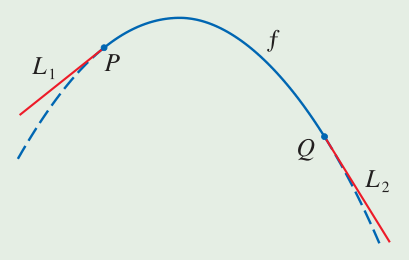
\includegraphics[width=\linewidth]{images/p0219_fig2.png}
    
    \vspace{12pt}
    \noindent
    \begin{minipage}[b]{0.90\linewidth}
      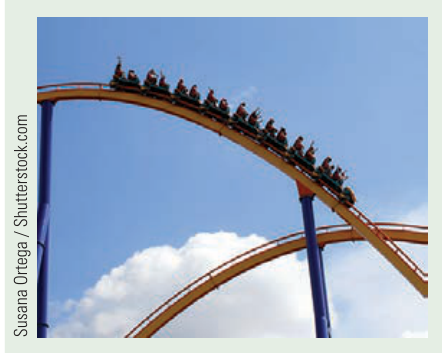
\includegraphics[width=\linewidth]{images/p0219_fig3.png}
    \end{minipage}%
    \begin{minipage}[b]{0.08\linewidth}
      \rotatebox{90}{\fontsize{4}{5}\selectfont\color{gray!80} Susana Ortega / Shutterstock.com}
    \end{minipage}
  \end{minipage}%
  \hfill
  \begin{minipage}[t]{0.66\textwidth}
    {\small
    Giả sử bạn được yêu cầu thiết kế đoạn dốc lên và dốc xuống đầu tiên cho một tàu lượn siêu tốc mới. Bằng cách nghiên cứu các bức ảnh chụp những chiếc tàu lượn yêu thích, bạn quyết định chọn độ dốc của đoạn dốc lên là $0{,}8$ và độ dốc của đoạn dốc xuống là $-1{,}6$. Bạn quyết định nối hai đoạn thẳng này $y = L_1(x)$ và $y = L_2(x)$ với một phần của đường parabol $y = f(x) = ax^2 + bx + c$, trong đó $x$ và $f(x)$ được tính bằng foot (ft). Để đường ray chuyển động êm thuận, hướng đi không được thay đổi đột ngột, vì vậy bạn muốn các đoạn thẳng $L_1$ và $L_2$ phải tiếp xúc với parabol tại các điểm chuyển tiếp $P$ và $Q$. (Xem hình vẽ.) Nhằm đơn giản hóa các phương trình, bạn quyết định đặt gốc tọa độ tại $P$.

    \vspace{5pt}
    \noindent\textbf{1.} 
    \begin{enumerate}[label=(\alph*), leftmargin=*, itemsep=2pt, topsep=1pt]
      \item Giả sử khoảng cách nằm ngang giữa $P$ và $Q$ là $100\text{ ft}$. Hãy viết các phương trình theo $a, b,$ và $c$ nhằm đảm bảo đường ray êm thuận tại các điểm chuyển tiếp.
      \item Giải hệ phương trình ở câu (a) để tìm $a, b,$ và $c$, từ đó xác định công thức cho $f(x)$.
      \item \graphicon\; Vẽ đồ thị của $L_1, f,$ và $L_2$ để kiểm chứng trực quan rằng các điểm chuyển tiếp thực sự êm thuận.
      \item Tìm độ chênh lệch độ cao giữa hai điểm $P$ và $Q$.
    \end{enumerate}

    \vspace{4pt}
    \noindent\textbf{2.} 
    Lời giải trong Bài toán 1 trông có vẻ \emph{êm thuận}, nhưng thực tế có thể không mang lại \emph{cảm giác} êm thuận vì hàm từng khúc [gồm $L_1(x)$ với $x < 0$, $f(x)$ với $0 \le x \le 100$, và $L_2(x)$ với $x > 100$] không có đạo hàm cấp hai liên tục. Vì vậy, bạn quyết định cải tiến thiết kế bằng cách chỉ sử dụng hàm bậc hai $q(x) = ax^2 + bx + c$ trên khoảng $10 \le x \le 90$ và nối nó với các đoạn thẳng bằng hai hàm bậc ba:
    \[
    \begin{aligned}
      g(x) &= kx^3 + lx^2 + mx + n && 0 \le x < 10 \\
      h(x) &= px^3 + qx^2 + rx + s && 90 < x \le 100
    \end{aligned}
    \]
    \begin{enumerate}[label=(\alph*), leftmargin=*, itemsep=2pt, topsep=1pt]
      \item Hãy lập hệ phương trình gồm 11 ẩn để đảm bảo rằng cả hai đạo hàm đầu tiên đều trùng khớp tại các điểm chuyển tiếp.
      \item \techicon\; Giải hệ phương trình ở câu (a) để tìm các công thức cho $q(x), g(x),$ và $h(x)$.
      \item Vẽ đồ thị của $L_1, g, q, h,$ và $L_2$, sau đó so sánh với đồ thị thu được ở Bài toán 1(c).
    \end{enumerate}
    }
  \end{minipage}
\end{tcolorbox}

\vfill
\noindent
\begin{center}
  \fontsize{5}{6}\selectfont\color{gray!80!black}
  Copyright 2021 Cengage Learning. All Rights Reserved. May not be copied, scanned, or duplicated, in whole or in part. WCN 02-200-203
\end{center}
